\cotefile{159}
\scanpage{1}
\figure{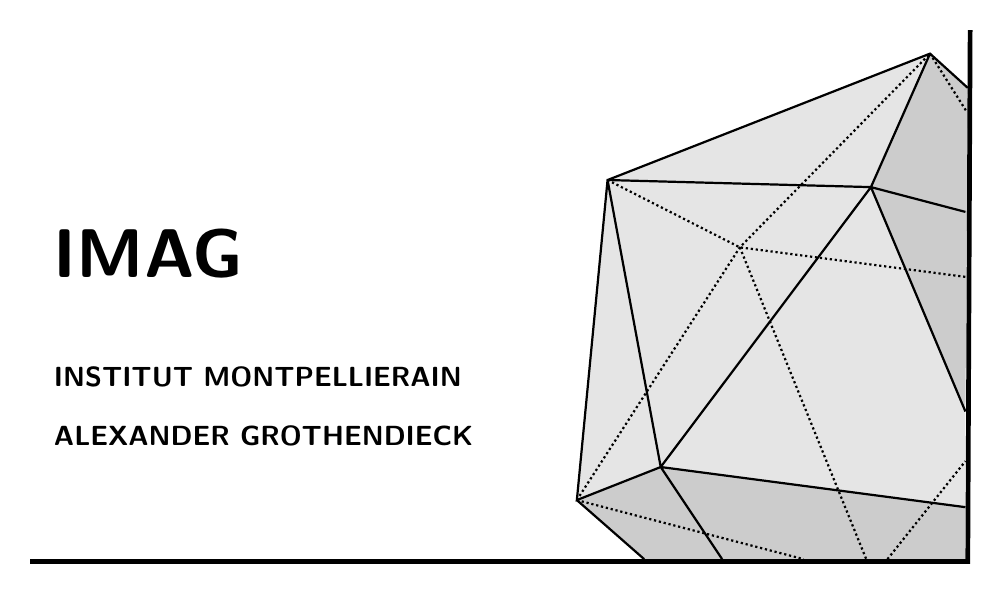
\begin{tikzpicture}[x=0.015cm,y=-0.015cm]
\node[anchor=west,font=\sffamily\bfseries\Huge] at (20,200) {IMAG};
\node[anchor=west,font=\sffamily\bfseries] at (20,305) {INSTITUT MONTPELLIERAIN};
\node[anchor=west,font=\sffamily\bfseries] at (20,355) {ALEXANDER GROTHENDIECK};
\fill[gray!20] (497,138)--(770,31)--(720,144)--(800,334)--(800,415)--(542,381)--(471,409)--cycle;
\fill[gray!40] (770,31)--(802,60)--(800,334)--(720,144)--cycle;
\fill[gray!40] (471,409)--(542,381)--(800,415)--(800,459)--(528,459)--cycle;
\draw[thick] (497,138)--(770,31)--(802,60) (770,31)--(720,144)--(497,138)--(471,409)--(542,381)--(497,138) (542,381)--(720,144)--(800,165) (720,144)--(800,334) (542,381)--(800,415) (471,409)--(528,459) (542,381)--(594,459);
\draw[thick,densely dotted] (497,138)--(609,195)--(800,220) (471,409)--(609,195)--(770,31) (609,195)--(716,459) (471,409)--(663,459) (734,459)--(800,376) (770,31)--(801,80);
\draw[line width=1.7pt] (8,461)--(802,461)--(804,11);
\end{tikzpicture}}
\scanpage{2}
% archive foliation: 1
Connexions projectives canoniques et uniformisation des courbes algébriques.

1. Connexions projectives

 a) $S$ schéma de base (disons). La donnée d'un fibré de Brauer-Severi \inserted{$P\deleted{\unsure{S}}$} sur $S$ (schém. propre et lisse/$S$ dont les fibres \inserted{géom.} sont des espaces projectifs) de dim relative \inserted{constante} $r$ revient à la donnée d'un torseur $\mathcal{T}$ sur $S$ de Groupe $\mathrm{GP}(r)_S$. La donnée d'un $P$ avec section marquée revient à se donner une restriction du groupe structural au sous-Groupe \inserted{de $\mathrm{GP}(r)_S$} qui fixe une section donnée de \deleted{\unsure{$\mathcal{O}$}} $P_0^r=\mathbb{P}(\mathcal{O}_S^{r+1})$, disons celle qui correspond au quotient $\mathcal{O}_S$ de $\unsure{\mathcal{O}_S^{r+1}}$ ``correspondant à la dernière coordonnée''. Ce sous-groupe s'identifie au groupe affine $\mathrm{Aff}(r\deleted{\unsure{+1}})_S$, produit \unsure{tordu}
\[
\mathrm{Aff}(r\deleted{\unsure{+1}})=\mathrm{GL}(r\deleted{\unsure{+1}}).\mathbb{E}^r
\]
où $\mathrm{GL}(r)$ opère sur $\mathbb{E}^r$ de la façon évidente.

[\unsure{les|Le} \inserted{Groupe des} automorphismes du Module $\mathcal{O}_S^{r+1}=\mathcal{O}_S^r\times\mathcal{O}_S$ \inserted{$=E_0\times L_0$} qui respectent la structure d'extension, modulo les $\unsure{\mathrm{mult}^{\mathrm{ons}}}$ scalaires, \deleted{\unsure{est}} est en fait celui des matrices
\diagram{\[
{}_{r+1}\left\{\left(\begin{array}{c|c}
\underbrace{A}_{r}&C\\ \hline
0&\unsure{1}
\end{array}\right)\right.\!\begin{array}{l}\big\}r\\{}\end{array}
\]}
avec $A$ \deleted{\unsure{scalaires}} dans $\mathrm{GL}(r)$, $C$ dans $\mathbb{E}^r$ ---]

On trouve aussi que la donnée de $(P,\sigma)$ \uline{équivaut} à celle d'une \inserted{structure d'}extension
\deleted{de}
\scanpage{3}
% archive foliation: 2
\diagram{\begin{tikzcd}[column sep=small]
0\arrow[r]&\Omega\arrow[r]&E\arrow[r]&\mathcal{O}_S\arrow[r]&0
\end{tikzcd}}

en ce sens que le \inserted{\unsure{contre}} foncteur qui à une telle extension fait correspondre $(P,\sigma)$ avec $P=\mathbb{P}(E)$ et $\sigma$ la section définie par le quotient \inserted{\unsure{inv.}} $\mathcal{O}_S$ de $E$, est une équivalence de catégories.

On trouve que les $\mathcal{O}_P/\mathcal{J}^{n+1}$ (où $\mathcal{J}$ est l'idéal de $\sigma(S)$ dans $P$) s'identifient comme $\mathcal{O}_S$-algèbres augmentées à
\[
\operatorname{Sym}^n(
\]
\scanpage{4}
% archive foliation: 3
\diagram{\begin{tikzcd}[column sep=small]
0\arrow[r]&\Omega\arrow[r]&E\arrow[r,"p"]&\mathcal{O}_S\arrow[r]&0
\end{tikzcd}}

$P=\mathbb{P}(E)$, $\sigma$ section définie par $p$, $\widehat P$ complété formel de $P$ le long de $\sigma$
\[
\widehat S=\mathcal{O}_{\widehat P}
\]
$\Omega$ opère \inserted{à g.} sur $\widehat S$ : car il opère sur l'extension (à g.) donc sur $(P,\sigma)$ et $\widehat P$ (à droite)

$L=\mathcal{O}_P(1)$, $\widehat L$ module inv. sur $\widehat S$

$\Omega$ opère à g. aussi sur $\widehat L$, de façon compatible avec opérations de $\Omega$ sur l'Anneau de scalaires $\widehat S$

Cas $E$ \inserted{extension} splittée (i.e. on a donné splitting $s:\mathcal{O}_S\to E$)
\[
E^0\simeq\Omega\times\mathcal{O}_S
\]
Alors \deleted{\unsure{$\widehat P(E^0)$} \unsure{par l'anneau comme} \illegible{2}},

\deleted{\illegible{1}} $\widehat P(S')\simeq$ Quotients inversibles \inserted{$L'$} de $E$, qui sur $S$ réd. coïncident avec le quotient donné $\mathcal{O}_S$ --- donc l'image dans $L'$ de la section $e$ de $\mathcal{O}_S\subset E$ est une base de $L'$, permettant d'identifier $L'$ à $\mathcal{O}_S$, de sorte que le quotient $\unsure{E}\to\deleted{\unsure{L'}}\inserted{\mathcal{O}_S}$ est défini par $(x,\lambda)\longmapsto\varphi(x)+\lambda$, où $\varphi:\Omega\to\mathcal{O}_S$ hom bien défini, de $\Omega$ dans nilradical \inserted{$N_S$}.

Donc
\[
\begin{aligned}
\widehat P^0&=\mathrm{V}(\Omega)^\wedge\quad\text{(complété formel le long de la section nulle)}\\
&=\operatorname{Spf}\underbrace{\widehat{\operatorname{Sym}}(\Omega)}_{\widehat S^0}
\qquad \widehat L^0\simeq\widehat S^0
\end{aligned}
\]
Il faut expliciter l'op. de $\Omega$ sur $\widehat S$. Soit $a\in\Omega(S)$.

Donc $a$ opère sur l'ext. $E$ par
\[
u_a(x,\lambda)=(x+\lambda a,\lambda)
\]
et si \deleted{\unsure{Donnons}} $\varphi:\Omega\to N_S$, définissant le \inserted{quotient} $\widetilde\varphi$ de $E$, \inserted{$\widetilde\varphi:E\xrightarrow{\text{épi}}\mathcal{O}_S$}, par $\widetilde\varphi(x,\lambda)=\varphi(x)+\lambda$, on aura le nouveau quotient par
\[
\begin{aligned}
\widetilde\varphi\circ u_a:\ (x,\lambda)&\longrightarrow\varphi(x+\lambda a)+\lambda\\
&=\varphi(x)+(1+\varphi(a))\lambda\\
&=(1+\varphi(a))\left(\frac{\varphi\deleted{\unsure{(x)}}}{1+\varphi(a)}(x)+\lambda\right),
\end{aligned}
\]
c'est aussi le quotient défini par \inserted{$(x,\lambda)\mapsto$} $\varphi^a(x)+\lambda$, donc
\scanpage{5}
% archive foliation: 4
moyennant l'identification $\widehat P\simeq\mathrm{V}(\Omega)^\wedge$, \unsure{le transport} de l'op. $u_a$ donne sur $\mathrm{V}(\Omega)^\wedge$
\[
\varphi^a=u_a^*(\varphi)=\frac{\varphi}{1+\varphi(a)}
\]
[De même, le morphisme induit $u_a^*$ sur les quotients inv. $L'\simeq\mathcal{O}_S$ \inserted{et $u_a^*(L')\simeq\mathcal{O}_S$} de $E=\Omega+\mathcal{O}_S$ est la multiplication par $1+\varphi(a)$]

Donc, \deleted{\unsure{$u_a^*$}} si $\varphi$ est identifié à un hom de $\widehat S=\widehat{\operatorname{Sym}}(\Omega)$ dans $\mathcal{O}_S$ (coïncidant sur $\Omega$ avec celui qu'on a déjà), on aura
\[
\varphi^a(\omega)=\frac{\varphi(\omega)}{1+\varphi(a)}=
\inserted{\varphi\left(\frac{\omega}{1+a}\right)=}
\varphi\left(\sum_{n\geq0}(-1)^n\omega a^n\right),
\]
donc
\[
\varphi^a(\omega)=\varphi(u_{a*}(\omega))
\]
où
\[
\boxed{u_{a*}(\omega)=\deleted{\unsure{\varphi}}\frac{\omega}{1+a}=\sum_{n\geq0}(-1)^n\omega a^n}
\]
\margin{d'où $\boxed{u_{a*}(f)=\dfrac{f}{(1+a)^n}\quad\text{si }\deg f=n}$}

Quel est l'hom canon. épi
\[
E\otimes_{\mathcal{O}_S}\widehat S\longrightarrow\widehat L\simeq\unsure{\widehat{\mathcal{O}}|\widehat S}
\]
(On a $E\simeq\Omega+\mathcal{O}_S$, donc
\[
E\otimes_{\mathcal{O}_S}\widehat S=\Omega\otimes_{\mathcal{O}_S}\widehat S+\widehat S
\]
).
\unsure{Sa} restriction au facteur $\widehat S\longrightarrow\mathrm{id}_{\widehat S}$
\deleted{$\pi(x,y)=$}

Sa restriction à l'autre facteur s'identifie à un $\mathcal{O}_S$-hom
\[
\Omega\longrightarrow\widehat S
\]
qui applique $\Omega$ dans $\widehat S^+$ --- c'est l'identité

Donc
\[
\pi(\omega\otimes f,g)=\omega f+g\qquad
\begin{gathered}\text{si }\omega\in\Omega(S)\\f,g\in\widehat S(S)\end{gathered}
\]
Quel est l'autom. de $\widehat L\simeq_{\mathcal{O}_S}\widehat S$ induit par l'autom. $u_a$ de la situation ? D'abord trouvons l'autom. $u_a^E$ de $E\otimes_{\mathcal{O}_S}\widehat S=\Omega\otimes_{\mathcal{O}_S}\widehat S+\widehat S$, il est \deleted{$u_{a*}^{\unsure{E}}\unsure{(\omega\otimes f,0\oplus g)}=$}
\scanpage{6}
% archive foliation: 5
écrivant un élém de $E\otimes\widehat S$ \inserted{loc sur $S$} comme somme d'élts de la forme
\[
\omega\otimes f+e\otimes g\qquad
\begin{gathered}\omega\in\Omega(S),\ f,g\in\widehat S(S)\\e\text{ la section marquée de }\mathcal{O}_S\subset E\end{gathered}
\]
\[
\begin{aligned}
u_{a*}^{\widehat E}(\omega\otimes f+e\otimes g)
&=u_a(\omega)\otimes u_{a*}(f)+u_a(\unsure{\omega|e})\otimes u_{a*}(g)\\
&=\omega\otimes u_{a*}(f)+(e+a)\otimes u_{a*}(g)\\
&=(\omega\otimes u_{a*}(f)+a\otimes u_{a*}(g))+e\otimes u_{a*}(g)
\end{aligned}
\]
On a donc
\[
\begin{aligned}
\pi(u_{a*}^{\widehat E}(\omega\otimes f+e\otimes g))
&=\omega u_{a*}(f)+a u_{a*}(g)+u_{a*}(g)\\
&=\omega u_{a*}(f)+(a+1)u_{a*}(g)
\end{aligned}
\]
tandis que
\[
\pi(\omega\otimes f+e\otimes g)=\omega f+g
\]
Il faut avoir
\diagram{\begin{tikzcd}
E\otimes\widehat S\arrow[r,"\pi"]\arrow[d,"u_{a*}^{\widehat E}"']&\widehat S\arrow[d,"u_{a*}^{\widehat L}"]\\
E\otimes\widehat S\arrow[r,"\pi"]&\widehat S
\end{tikzcd}}
\unsure{Or}, $\pi\circ u_{a*}^{\widehat E}=u_{a*}^{\widehat L}\circ\pi$, et faisant $\unsure{\omega\otimes f=0|\omega f=0}$, on trouve eq.
\[
\boxed{u_{a*}^{\widehat L}(g)=(a+1)u_{a*}(g)}
\quad\left(=\frac{g}{(1+a)^{n-1}}\text{ si }\deg g=n\right)
\]
Vérifions \unsure{ceci} en général par acquit de conscience.
\[
\begin{aligned}
u_{a*}^{\widehat L}\pi(\omega\otimes f+e\otimes g)
&=(a+1)u_{a*}(\omega f+g)\\
&=(a+1)(\underbrace{u_{a*}(\omega)}_{\frac{\omega}{\unsure{1-a|1+a}}}u_{a*}(f)+u_{a*}(g))\\
&=\\
&=\omega u_{a*}(f)+(a+1)u_{a*}(g)\qquad\text{OK !}
\end{aligned}
\]
Si on revient au cas général d'une extension quelc. de $\mathcal{O}_S$ par $\Omega$, définie par un torseur $\mathcal{T}$ sous $\Omega$, on trouve donc
\[
\left\{\begin{aligned}
\widehat S&=\deleted{\unsure{\widehat{\operatorname{Sym}}(\Omega)\wedge_{(\Omega,u)}}}\mathcal{T}\wedge_{(\Omega,u_{a*})}\widehat{\operatorname{Sym}}(\Omega)\\
\widehat L&=\mathcal{T}\wedge_{(\Omega,u_{a*}^{\widehat L})}\widehat{\operatorname{Sym}}(\Omega).
\end{aligned}\right.
\]
\deleted{Comment calculer les extensions successives $\mathcal{J}^n/\mathcal{J}^{n+2}$ ext. de $\operatorname{Sym}^n\Omega$ par $\operatorname{Sym}^{n+1}\Omega$}
\scanpage{7}
% archive foliation: 6
\uline{Conséquence} : Si $\widehat{\mathcal{J}}$ est l'idéal d'augm. de $\widehat S$, qu'on filtre $\widehat{\mathcal{J}}$-adiquement, on aura
\[
\operatorname{gr}^1_{\widehat{\mathcal{J}}}(\widehat S)\simeq\Omega
\]
d'où
\[
\operatorname{gr}^{\bullet}_{\widehat{\mathcal{J}}}(\widehat S)\simeq\operatorname{Sym}^{\bullet}(\Omega)
\]
D'autre part, $\mathcal{J}^n/\mathcal{J}^{n+2}$ est une ext. de $\operatorname{gr}^n\simeq\operatorname{Sym}^n(\Omega)$ par $\operatorname{gr}^{n+1}=\operatorname{Sym}^{n+1}(\Omega)$ qu'on va calculer, en notant que l'op. $u_{a*}$ de $a$ sur \deleted{\unsure{$\operatorname{gr}$}} $\widehat{\mathcal{J}}^{(0)n}/\widehat{\mathcal{J}}^{(0)n+2}$ est donnée par
\[
\deleted{\unsure{\sum\omega_1\cdots\omega_n+\sum\omega'_1\cdots\omega'_{n+1}\longrightarrow}}
\]
\[
\begin{aligned}
\underset{\deg n}{f}+\underset{\deg n+1}{g}
&\longrightarrow\frac{f}{(\unsure{1+a|1-a})^n}+\frac{g}{(\unsure{1-a|1+a})^{n+1}}\\
&\unsure{=}f\unsure{-|+}naf+g+\text{termes de degré }\geq n+2
\end{aligned}
\]
Soit donc
\diagram{\begin{tikzcd}[column sep=large]
\Omega\arrow[r,"v_n"]&\underline{\operatorname{Hom}}(\operatorname{Sym}^n\Omega,\operatorname{Sym}^{n+1}\Omega)\arrow[d,phantom,"\simeq"]\\
&\text{Aut d'ext de }\widehat{\mathcal{J}}^{0n}/\widehat{\mathcal{J}}^{0n+2}
\end{tikzcd}}
défini par
\[
v(a)(f)=af.
\]
\deleted{on a alors}
(\uline{NB}. C'est un iso si $\Omega$ inversible). On a alors
\[
\mathcal{T}\times_{\Omega}[\underline{\operatorname{Hom}}(\operatorname{Sym}^n\Omega,\operatorname{Sym}^{n+1}\Omega),-nv_n]
\]
qui donne l'extension.
\scanpage{8}
% archive foliation: 7
Soit $X$ schéma lisse sur $S$, \deleted{Un} $n$ un entier $\geq0$. Une \uline{$n$-connexion projective} sur $X$ (rel. à $S$) est la donnée

 a) d'un fibré de B.S $P$ sur $X$ avec une section, ou ce qui revient au même, une extension
\diagram{\begin{tikzcd}[column sep=small]
0\arrow[r]&\Omega\arrow[r]&E\arrow[r]&\mathcal{O}_X\arrow[r]&0
\end{tikzcd}}
de Modules loc. libres sur $X$, ou encore un couple $(\Omega,\mathcal{T})$ de $\Omega$ loc. libre sur $X$ et $\mathcal{T}$ un $\Omega$-tors.

 b) Un \inserted{$X$-}isom des voisinages inf. d'ordre $n$ de la diagonale de $X\times_S X$ avec le vois. d'ordre $n$ de $\sigma$ dans $P$, ou ce qui revient au même, un isom de \inserted{$\mathcal{O}_X$-}Algèbres augmentées
\[
P^n_{X/S}\overset{\alpha_n}{\simeq}\mathcal{O}_{\widehat P}/\widehat{\mathcal{J}}^{n+1}
\quad(\simeq\mathcal{T}\times_{\Omega}\operatorname{Sym}^{\bullet}(\Omega)/\operatorname{Sym}^{+}(\Omega)^{n+1})
\]
(où $\widehat P$ est le complété formel de $P$ le long de $\sigma(X)$, et $\widehat{\mathcal{J}}$ l'Idéal de déf. de la section $\sigma$).

Pour $n=0$, la donnée b est vide. Pour $n=1$, elle revient à un iso
\[
(*)\qquad\Omega\simeq\Omega^1_{X/S}
\]
\margin{donc le rang de $\Omega$ en tt pt doit être la dim rel de $X$ sur $S$ en ce pt.}

Pour $n=2$, la structure de $P^2_{X/S}$ est entièrement déterminée par la structure d'extension de $\Omega^1_{X/S}$ par $\operatorname{Sym}^2\Omega^1_{X/S}$, \deleted{\unsure{qui doit|qui définit}} \inserted{i.e.} \deleted{\unsure{d'une connex}} un torseur sous $\underline{\operatorname{Hom}}_{\mathcal{O}_S}(\Omega^1_{X/S},\operatorname{Sym}^2\Omega^1_{X/S})$ lequel doit donc être muni d'un iso avec le torseur déduit de $\mathcal{T}$ sous $\Omega$, de
\diagram{\begin{tikzcd}[column sep=large]
\Omega\arrow[r,"-v_1"]&\underline{\operatorname{Hom}}(\Omega,\operatorname{Sym}^2(\Omega))\arrow[d,phantom,"\simeq"]\\
&\underline{\operatorname{Hom}}(\Omega^1_{X/S},\operatorname{Sym}^2\Omega^1_{X/S})
\end{tikzcd}}
et l'iso découlant de l'iso $\alpha$. Donc si la dim relative
\scanpage{9}
% archive foliation: 8
$r$ de $X$ sur $S$ est $1$, \deleted{\unsure{on a}} (alors $v_1,-v_1$ des iso) ou $r+1$ inv. sur $S$ (alors $v_1,-v_1$ ont des inv. à g.), \deleted{le} \inserted{$\Omega$ et $\Omega$-}torseur $\mathcal{T}$ est canoniquement déterminé par $X$, par $\Omega\simeq\Omega^1_{X/S}$ et $\unsure{\alpha_n}$.

On définit de même une $\infty$-connexion \inserted{projective} (Remarque : est-il vrai que pour une telle $\infty$-conn. proj, $\mathcal{T}$ est can. déterminé par $X/S$, sans condit. de dim ni de car. ?)

Notons que \inserted{la pro-$\mathcal{O}_X$-alg} $P^\infty_{X/S}$ a une \deleted{connexion} \inserted{stratification} \deleted{plate} canonique $\Delta$ (\deleted{\unsure{donc induit une connexion}} \inserted{ne respectant pas l'}augmentation $P^\infty_{X/S}\to\unsure{\mathcal{O}_X|\mathcal{O}_{X/S}}$ !), donc si $X$ est muni d'une $\infty$-connexion projective, alors \inserted{la pro-$\mathcal{O}_X$-alg} $\widehat P$ i.e. $\widehat S$ se trouve sur $X$ muni d'une \deleted{$\infty$-connexion} \inserted{stratification} \deleted{correspondante} \inserted{$\Delta'$}. On dit que la $\infty$-conn. projective est \inserted{plate (ou} \uline{intégrable}) si $\Delta'$ provient d'une \deleted{$\infty$-connexion} stratification de $P=\mathbb{P}(E)$ (en oubliant \unsure{pour} la section marquée à présent) laquelle sera dès lors uniquement déterminée (et qualifiée de ``canonique'').

Cette condition étant locale sur $X$, pour l'exprimer on peut supposer que $X$ est muni de ``coordonnées locales'' $f_1\ldots f_r$ (\unsure{sections relat. à un $\alpha$ sur $S$}). Dès lors
\[
P^\infty_{X/S}\simeq\mathcal{O}_S[[\delta f_1,\ldots,\delta f_r]]
\]
et
\[
\Delta:P^\infty_{X/S}\longrightarrow P^\infty_{X/S}\widehat\otimes_{\mathcal{O}_S}P^\infty_{X/S}
\simeq P^\infty_{X/S}(P^\infty_{X/S})\simeq P^\infty_{X/S}[[\overline{\delta f_1},\ldots,\overline{\delta f_r}]]
\]
\[
\Delta(\delta f_i)=\delta(f_i)\otimes1+1\otimes\delta(f_i)=\delta f_i+\overline{\delta f_i}
\]
\margin{\[
M\otimes P^n_{X/S}\longrightarrow P^n_{X/S}\otimes M
\]
\deleted{un} $P^n_{X/S}$-linéaire qui est \deleted{\unsure{bij}} \inserted{par réduction}
i.e.
\[
M\xrightarrow{\Delta}P^n_{X/S}\otimes M
\]
$\mathcal{O}_S$-lin par stratification. id. après réduction \inserted{sur 2ème facteur}
\[
\Delta(m)=m+\sum
\]}

On peut supposer l'extension $E$ splittée, donc $\widehat S\simeq\widehat{\operatorname{Sym}}(\Omega)$ et comme $\Omega\simeq\Omega^1_{X/S}\simeq\mathcal{O}_S^r$,
\[
\widehat S\simeq\mathcal{O}_S[[T_1,\ldots,T_r]]
\]
La $\infty$-conn. projective est
\scanpage{10}
% archive foliation: 9
donnée par les images des $T_i$ dans $P^\infty_{X/S}$, des
\[
\left.\begin{gathered}
F_i\in\Gamma_S P^\infty_{X/S}\unsure{\simeq}\Gamma_S\mathcal{O}_S[[\delta f_1,\ldots,\delta f_r]]\\
F_i=\delta f_i+G_i\qquad G_i\text{ d'ordre }\geq2
\end{gathered}\right\}\quad1\leq i\leq r
\]
ou inversement par les images des $\delta f_i$, soit
\[
\left.\begin{gathered}
\Phi_i\in\Gamma\deleted{\widehat{\operatorname{Sym}}}\mathcal{O}_S[[T_1,\ldots,T_r]]\\
\Phi_i=T_i+\Psi_i\qquad(\Psi_i\text{ d'ordre }\geq2)
\end{gathered}\right\}\quad1\leq i\leq r
\]
On a donc la \deleted{connexion} \inserted{stratification} sur $\mathcal{O}_S[[T_1,\ldots,T_r]]$
\[
\mathcal{O}_S[[T_1,\ldots,T_r]]=\widehat S\xrightarrow{\Delta'}P^\infty_{X/S}\otimes\widehat S=P^\infty_{X/S}(\widehat S)\simeq P^\infty_{X/S}[[T_1,\ldots,T_r]]
\]
déduite par transport de structure de celle de $P^\infty_{X/S}$. Il faut donner les images des $T_i$ dans $P^\infty_{X/S}[[T_1,\ldots,T_r]]$, ce sera l'image de
\[
\Delta(\deleted{\unsure{F_i}}\delta f_i+G_i)\in\Gamma P^\infty_{X/S}\widehat\otimes P^\infty_{X/S}
\]
dans $\Gamma P^\infty_{X/S}\otimes\widehat S$, déduite de $\longrightarrow$ obtenue par l'iso. $\omega:P^\infty_{X/S}\to\widehat S$. Posant
\scanpage{11}
% archive foliation: 10
\diagram{\begin{tikzcd}X\arrow[d,"f"']\\S\end{tikzcd}}
propre lisse dim rel. 1 fibres connexes
\[
\Omega^1_{X/S}=\omega\qquad f_*(\omega)=\Omega\qquad
\mathbf{R}^1f_*(\Omega^*_{X/S})=\mathcal{DR}
\]
\[
\mathrm{R}^1f_*(\mathcal{O}_X)\simeq\check\Omega\simeq t
\]
\diagram{\begin{tikzcd}[column sep=small]
0\arrow[r]&\Omega\arrow[r]&\mathcal{DR}\arrow[r]&\check\Omega\arrow[r]&0
\end{tikzcd}}
\margin{autodualité
\deleted{$\mathcal{DR}\times\mathcal{DR}\longrightarrow\mathcal{O}_S$ \uline{alternée}}}
\deleted{le faisceau des \unsure{splittings} \unsure{de} $\mathcal{DR}\to\check\Omega\to0$ \unsure{est un espace}}
\diagram{\begin{tikzcd}[column sep=small]
\deleted{0}\arrow[r]&\deleted{\unsure{\check\Omega\otimes\check\Omega}}\arrow[r]&\deleted{\unsure{\Sigma}}\arrow[r]&\deleted{\mathcal{O}_S}\arrow[r,dash]&\deleted{0}
\end{tikzcd}}
\[
\mathcal{DR}\times\mathcal{DR}\xrightarrow[\varphi]{\text{alterné}}\mathcal{O}_S
\qquad(=\mathbf{R}^2f_*(\Omega^*_{X/S})\simeq\mathrm{R}^1f_*(\Omega^1_{X/S}))
\]
\deleted{nulle sur $\Omega\times\Omega$, d'où}
l'orthogonal de $\Omega$ est $\Omega$, :
\[
\deleted{\unsure{\mathcal{DR}}\quad\Omega\otimes\check\Omega}
\qquad\bigwedge^2\mathcal{DR}\xrightarrow[\varphi]{}\mathcal{O}_S
\]
\diagram{\begin{tikzcd}[column sep=small]
0\arrow[r,dash]&\Omega\arrow[r,dash]\arrow[d,"\mathrm{id}"']&\mathcal{DR}\arrow[r,dash]\arrow[d,"\unsure{\sim}"]&\check\Omega\arrow[r,dash]\arrow[d,"\mathrm{id}"]&0\\
0\arrow[r,dash]&\Omega\arrow[r,dash]&\check{\mathcal{DR}}\arrow[r,dash]&\check\Omega\arrow[r]&0
\end{tikzcd}}
\unsure{I.e.} on connaît déjà l'accouplement sur $\Omega\times\mathcal{DR}$ et $\mathcal{DR}\times\Omega$ --- l'indétermination est dans \deleted{\unsure{$\Omega$}} $\operatorname{Hom}(\check\Omega\otimes\check\Omega,\mathcal{O}_S)=\Omega\otimes\Omega$ et $=$ (puisqu'il s'agit de formes alternées) dans $\bigwedge^2\Omega$
\diagram{\begin{tikzcd}[column sep=large]
0\arrow[r,dash,"\bigwedge^2\Omega"]&\uline{\mathrm{Fil}^2}\arrow[r,dash,"\Omega\otimes\check\Omega"]&\mathrm{Fil}^1\arrow[r,dash,"\bigwedge^2\check\Omega"]\arrow[dr,"\unsure{\text{éval}}"']&\bigwedge^2\mathcal{DR}\arrow[d,dashed,"\varphi"]\\
&&&\mathcal{O}_S
\end{tikzcd}}
Pour un splitting de $\mathcal{DR}$ par $q:\check\Omega\to\mathcal{DR}$, on aura comme matrice de $\varphi$ pour la décomposition $\mathcal{DR}\overset{q}{\simeq}\Omega\oplus\check\Omega$
\diagram{\[
\begin{pmatrix}0&+\mathrm{id}\\-\mathrm{id}&\varphi_0\end{pmatrix}
\]}
où $\varphi_0$ est une forme alternée sur $\check\Omega$. Pour un autre choix $q'(t)=q(t)+u(t)$ ($u:\check\Omega\to\Omega$) on aura
\[
\begin{aligned}
\varphi'_0(t,t')&=\varphi(q(t)+u(t),q(t')+u(t'))\\
&=\varphi_0(t,\unsure{t'})\unsure{-|+}\langle t,u(t')\rangle\unsure{+|-}\langle t',u(t)\rangle\deleted{\unsure{+}}
\end{aligned}
\]
\scanpage{12}
% archive foliation: 11
Si on s'intéresse aux splittings pour lesquels $\varphi'_0=0$, on voit que c'est une condition lin. et on trouve un fibré torseur sous $\Gamma^2\Omega$ (formes symétriques sur $\check\Omega$)
\diagram{\begin{tikzcd}[column sep=small]
0\arrow[r,dash]&\Gamma^2\Omega\arrow[r,dash]&\overline\Sigma\arrow[r]&\mathcal{O}_S\arrow[r]&0
\end{tikzcd}}
\margin{torseur des splittings hyperboliques de \deleted{\unsure{$\mathcal{O}_S$}} $\mathcal{DR}$}
(Il est induit par un torseur analogue sur le schém. modulaire pour les \deleted{\unsure{jacobiennes}} \inserted{VA} \unsure{via} jacobiennes).

On a connexion \inserted{plate} (si $S$ sur $T$)
\[
\mathcal{DR}\longrightarrow\mathcal{DR}\otimes\Omega^1_{S/T}
\]
en général non compatible avec la filtration, le défaut de compatibilité s'exprimant par
\[
\Omega\longrightarrow\check\Omega\otimes\Omega^1_{S/T}
\]
d'où
\[
\mathcal{T}_{S/T}\longrightarrow\check\Omega\otimes\check\Omega
\]
(qui est \deleted{\illegible{1}}, induit par la flèche analogue pour jacobiennes $f$, et sur la variété modulaire pour les VA \inserted{princ.} c'est un iso; ici donc, \deleted{\unsure{donc}} si $S/T$ est modulaire pour les courbes de genre $g$, ce sera un \uline{mono} sauf pour les courbes hyperelliptiques), qui en fait se factorise par
\[
\mathcal{T}_{S/T}\longrightarrow\Gamma^2\check\Omega
\]
(sur le schém. modulaire pour les VA \uline{polarisées} avec pol. \deleted{\unsure{pri}} première aux car. de $T$, ce sera encore un iso ---)

Sur $X$ \inserted{($g\geq2$)}, on a un fibré lin. provenant d'un sous-fibré de corang 1 (dans \inserted{$\Omega_X$} $H^0(X,\Omega_X)$) (\deleted{sections de} formes diff. de degré 1 s'annulant au \uline{pt déf.}),
\margin{\diagram{\begin{tikzcd}[column sep=small]
0\arrow[r]&\Omega'_X\arrow[r]&\Omega_X\arrow[r]&\omega_X\arrow[r]&0
\end{tikzcd}}}
\diagram{\begin{tikzcd}[column sep=small]
0\arrow[r]&\Omega'_X\arrow[r,hook]&\Omega_X\arrow[r,hook]&{\Omega'_X}^{\perp}\arrow[r,hook]& (\mathcal{DR})_X
\end{tikzcd}}
\margin{dans $\mathcal{DR}_X$}
\scanpage{13}
% archive foliation: 12
\deleted{$\operatorname{Hom}(\Omega$}
\margin{splittings $\varphi$-admissibles}
\diagram{\begin{tikzcd}[column sep=large]
 & \varphi \\
\text{Splittings de }\mathcal{DR}\arrow[r] & \begin{gathered}\text{formes alternées}\\\text{admissibles}\\\text{sur }\mathcal{DR}\end{gathered}\arrow[u]
\end{tikzcd}}
\diagram{\begin{tikzcd}[column sep=large]
0\arrow[r]&\Gamma^2\Omega\arrow[r]\arrow[d,"{\substack{\text{Épi (cas non hyperelliptique)}\\(\text{car.}\ne2)}}"]&\Omega\otimes\Omega\arrow[r]&\bigwedge^2\Omega\arrow[r]&0\\
&f_*(\omega^2)\simeq\Omega^{1\deleted{\unsure{0}}}_{S/T}
\end{tikzcd}}
\[
\frac{g(g+1)}2-(3g-3)=\frac12\bigl(\underbrace{g^2-5g+6}_{(g-2)(g-3)}\bigr)=\frac12(g-2)(g-3)
\]
\diagram{\begin{tikzcd}
0\arrow[r]&\mathcal O_X\arrow[r]&\unsure{\mathcal V_0}\arrow[r,dash]&\omega^{-1}\arrow[r,dash]&0
\end{tikzcd}}
\[
\deleted{\unsure{\varphi}}\qquad \bar E\otimes_{\mathcal O}P-\bar E
\]
\[
2-2g
\]
\[
P^\infty_{X/S}\qquad\underbrace{\Omega\quad\Omega^2}\quad\Omega^3
\]
\diagram{\begin{tikzcd}
0\arrow[r]&\omega^2\arrow[r]&P^{\unsure{3+|2+}}_{X/S}\arrow[r]&\omega\arrow[r,dash]&0
\end{tikzcd}}
\margin{$X^n$}
\diagram{\begin{tikzcd}
0\arrow[r,dash]&f_*(\omega^2)\arrow[r]\arrow[d,phantom,"\simeq" description]&f_*(P^{\unsure{3+|2+}}_{\unsure{X/S}})\arrow[r,dash]&f_*(\omega)\arrow[r]\arrow[d,phantom,"\Vert" description]&0\\
&\Omega^1_{S/T}&&\Omega
\end{tikzcd}}
\margin{$\mathcal J\subset A\otimes_a A\longrightarrow A$\par
$\mathcal J/\mathcal J^2$\par
$x\otimes y-y\otimes x$}
\[
\deleted{P^\infty(\operatorname{Sym}^\bullet(\Omega))}
\qquad P^{\unsure{0|\infty}}(\omega^n)
\]
\[
\deleted{\operatorname{Gr}}\quad \deleted{f_*(\omega^i)\cdot\mathcal O_S}\qquad P^\infty(\omega^n)
\]
\diagram{\begin{tikzcd}
\deleted{P^\infty(\operatorname{Sym}^\bullet(\Omega))}_{\unsure{\omega}}\arrow[dr]\\
\omega\otimes P^\infty &P^\infty\otimes\omega
\end{tikzcd}}
\[
\uline{M}\otimes P^\infty\unsure{\mathcal O}\qquad
R^1f_*(M\otimes\omega^n)=0\quad\text{si }\unsure{d_M\cdot n\ge1}
\]
\deleted{\unsure{Puis}}\quad\deleted{$\unsure{\omega\otimes P^\infty}$}
\[
S^i=f_*P^\infty(\omega^{\unsure{n|i}})=f_*(\omega^{\unsure{n|i}}\otimes P)\qquad\text{une}
\]
\unsure{$S^0$-algèbre graduée}\par
\deleted{\unsure{et d'algèbre}}\par
\unsure{a-graduée} (\unsure{ou} $f_*(\Sigma^\bullet\omega^n)=\Sigma^\bullet$)
\unsure{graduée associée} :
\diagram{\begin{tikzcd}
\Sigma^*\arrow[r]&S^*\arrow[l,bend right=45]\arrow[d,bend left=45]\\
&R^*\arrow[u]
\end{tikzcd}}
\[
\Sigma^*\otimes R^*\qquad \operatorname{gr}S^*\simeq\sum_{\unsure{n,q}}f_*(\omega^{\unsure{n+q}}).
\]
\scanpage{15}
% archive foliation: 14
Fixons nous un genre $g$ ($\ge2$ au besoin) et un foncteur rigidifiant (p.ex. de Jacobi d'échelon convenable), pour les courbes algébriques relatives sur une base donnée (disons travaillant sur la \deleted{\unsure{base}}\inserted{multiplicité} modulaire des courbes de genre $g$ -- lisses, propres, geom. connexes -- la catégorie fibrée qu'il définit, ou la multiplicité modulaire, est notée $M_g$.

Considérons
\[
M_g^{\unsure{\xi|\zeta}}(S)=\begin{gathered}
\text{courbes algébriques relatives }X\text{ de \uline{genre} }g\\
\text{sur }S,\ \text{\uline{munies} d'un fibré en droites projectives}\\
P\text{ sur }X,\text{ avec une }\unsure{\xi|\zeta}\text{-structure (conn. lin.)}
\end{gathered}
\]
\margin{$S$ : schéma de base \uline{de car. $0$}}
rel. à $S$, telle que $\forall s$ pt. géom de $S$, \inserted{dans} $P_s$ sur $X_s$ \unsure{on n'ait point} $\unsure{\xi|\zeta}$-réduction du groupe structural ni à un $G_{\unsure{a|0}}\subset GP(1)$, ni à un $G_m\subset GP(1)$

(i.e. $P$ n'est isomorphe à aucun des $2$ types ``\uline{dégénérés}'' suivants\unsure{\ldots\ldots})

\uline{Prop} Soit $X$ \deleted{courbe}\inserted{schéma} algébrique connexe sur $k$ alg. clos, \deleted{\unsure{de car. $0$}}, $P$ un $\unsure{\xi|\zeta}$-fibré en droites projectives sur $X$, conditions équivalentes
\[
\begin{array}{ll}
a)&\operatorname{Aut}^{\unsure{\xi|\zeta}}(P)=1\\
b)&\operatorname{Aut}^{\unsure{\xi|\zeta}/k}_{X/k}(P)\text{ (qui est un grp alg}\inserted{\subset GP(1)_k}\text{) est de dim }0
\end{array}
\]
\unsure{c)} $P$ n'est pas de l'un des deux types

$\alpha)$ associé à un $G_m$-$\unsure{\xi|\zeta}$ fibré, i.e. à un $\unsure{\xi|\zeta}$-faisceau inversible $\Omega$, on prend la clôture projective de $V(\Omega)$, i.e. $P(\Omega+\mathcal O)$

$\beta)$ associé à un $G_a$-$\unsure{\xi|\zeta}$-fibré, i.e. à une $\unsure{\xi|\zeta}$ extension
\diagram{\begin{tikzcd}
0\arrow[r,dash]&\mathcal O_X\arrow[r]&E\arrow[r]&\mathcal O_X\arrow[r]&0
\end{tikzcd}}
(pour les $\unsure{\xi|\zeta}$-structures triviales sur $\unsure{\mathcal O|E}$) on prend $P(E)\simeq$ clôture projective du torseur image inverse de $1$
\margin{l'\unsure{intersection} de ces deux types est $\unsure{\xi|\zeta}$-structure \uline{\unsure{triviale}} (\unsure{i.e.} $\unsure{\xi|\zeta}$ \unsure{torseurs})}
\scanpage{16}
% archive foliation: 15
\unsure{\deleted{Si $X$ est une courbe alg. de genre $g$,}}
\inserted{\unsure{Si $X$ courbe algébrique lisse} \inserted{propre} de genre $g$\deleted{$\unsure{\ge0}$}}, et $k$ de car. nulle, conditions équivalentes
\[
\begin{array}{ll}
d)&\dim H^1_{DR}(X,\unsure{\mathfrak g})=6g-6\quad\deleted{\unsure{(si $g$}}\\
d')&H^0_{DR}\deleted{\unsure{\xi}}(X,\unsure{\mathfrak g})\ (=H^{0\unsure{\xi|\zeta}}(X,\unsure{\mathfrak g}))=0\\
d'')&H^2_{DR}(X,\unsure{\mathfrak g})\ (=H^{2\unsure{\xi|\zeta}}(X,\unsure{\mathfrak g}))=0
\end{array}
\]
\margin{(conditions jamais vérifiées si $g=0$ -- et pour cause !)}

[\uline{NB} On a $\unsure{\mathfrak g}\simeq\check{\unsure{\mathfrak g}}$ (Killing) donc
\[
(*)\quad H^0_{DR}(X,\unsure{\mathfrak g})\simeq H^2_{DR}(X,\unsure{\mathfrak g})^\vee
\]
(\unsure{d'où équiv. de $d'$ et $d''$}) et formule de EP
\[
\begin{aligned}
(**)\quad\chi^{\unsure{\xi|\zeta}}_{DR}(X,\unsure{\mathfrak g})
&=\sum(-1)^i\dim H^i_{DR}(X,\unsure{\mathfrak g})
=\underbrace{3}_{\operatorname{rg}\unsure{\mathfrak g}}\ \underbrace{\chi^{\unsure{\xi|\zeta}}(X,\mathcal O_X)}_{2-2g}\\
&=\deleted{\unsure{6g}}6-6g
\end{aligned}
\]
donc, combinant avec $(*)$
\[
(***)\quad \dim H^1_{DR}(X,\unsure{\mathfrak g})=2\dim H^0_{DR}(X,\unsure{\mathfrak g})+(6g-6)
\]
\margin{\deleted{\unsure{dim gr. $G$}}}
d'où l'équivalence de $d')$ avec $d)$.

Enfin, on sait
\[
H^0_{DR}(X,\unsure{\mathfrak g})\simeq\uline{\operatorname{Lie}}\operatorname{Aut}^{\unsure{\xi|\zeta}}_{X/k}(P)
\]
d'où l'équivalence de $d')$ avec $b)$, et la formule intéressante
\[
\begin{aligned}
\dim\underbrace{H^1_{DR}(X,\unsure{\mathfrak g})}_{\substack{\text{espace tangent}\\\text{à l'espace modulaire}\\M_g^{\unsure{\xi|\zeta}}\text{ au pt correspondant}\\\text{à }(X,P,\unsure{\xi|\zeta})}}
&=2\dim\operatorname{Aut}^{\unsure{\xi|\zeta}}_{X/k}(P)+6g-6\\
&=2\bigl(\dim\operatorname{Aut}^{\unsure{\xi|\zeta}}_{X/k}(P)+3g-3\bigr)
\end{aligned}
\]

\uline{NB} La condition $d')$ implique que $M_g^{\unsure{\xi|\zeta}}$ ``n'a pas d'autom. infinitésimaux'', $a)$ qu'il ``n'a pas d'autom. finis'', donc ensemble que $M_g^{\unsure{\xi|\zeta}}$ est ``\uline{rigide}'' -- tout comme $M_g$ -- donc un foncteur représentable ! La condition $d'')$ implique que $M_g^{\unsure{\xi|\zeta}}$ est \inserted{form.} lisse sur $M_g$, et $d)$ que sa dim relative sur $M_g$ est $6g-6$.

Sans doute peut-on prouver la représentabilité relative (du moins au sens espaces alg. d'Artin)
\scanpage{17}
% archive foliation: 16
$X$ courbe analytique connexe compacte genre $g\ge\unsure{2|1}$

$M_g^{\unsure{\xi|\zeta}}(X)$ espace modulaire pour les fibrés projectifs analytiques à connexion plate sur $X$, ``sans automorphismes''. C'est l'espace analytique associé à un schéma (de t.f. ?) sur $\mathbb C$, \deleted{mais} lisse de dim $6g-6$, mais on le regarde pt de vue analytique. Il est alors can. isomorphe (une fois choisi pt base $x\in X$) à l'espace des représentations
\diagram{\begin{tikzcd}
\pi\arrow[r,"\rho"]\arrow[d,phantom,"\Vert" description]&GP(1,\mathbb C)=H\\
\pi_1(X,x)
\end{tikzcd}}
\deleted{\unsure{telles}} que $\operatorname{Cent}(\rho)=\{e\}$, \deleted{\unsure{\#}} \unsure{quotienté} par $H$ opérant par composition avec aut. intérieurs
\[
M_g^{\unsure{\xi|\zeta}}(X)\simeq {}_H\!\backslash\uline{\operatorname{Hom}}^!_{\operatorname{gr.}\deleted{\unsure{\mathrm{cont}}}}(\pi,H)\deleted{\unsure{/H}}
\]
où le $!$ désigne le sous-ens. des $\rho\in\uline{\operatorname{Hom}}_{\operatorname{gr}}(\pi,H)$ dont le stabilisateur dans $H$ est réduit à $1$.

[\uline{NB} Il est immédiat de faire de $\uline{\operatorname{Hom}}_{\operatorname{gr}}(\pi,H)$ un espace algébrique (de façon que pour $g\in\pi$, les morphismes $\rho\longmapsto\rho(g)$ soient algébriques), de façon que $H$ y opère algébriquement. Mais l'iso précédent \uline{n'est pas} \inserted{\uline{sans doute}} algébrique !]
\margin{$?\ \big|$}
L'interprétation ``géom.'' de $\operatorname{Hom}^!$ lui-même est : on classifie les couples $(P,c,\varphi)$, $(P,c)$ un
\scanpage{18}
% archive foliation: 17
$\unsure{\xi|\zeta}$-fibré en droites projectives et $\varphi:P^1(\mathbb C)\longrightarrow P_x$ un iso. L'opération de $H$ dessus est \unsure{l'évidente}.

Or le groupe $\operatorname{Aut}(\pi)$ opère \inserted{à droite} sur $\uline{\operatorname{Hom}}(\pi,H)$ ; \deleted{et} si $u\in\operatorname{Aut}(\pi)$, $\rho\in\uline{\operatorname{Hom}}(\pi,H)$, on pose $\rho.u=\rho\circ u$ \inserted{(les op. commutent à celles de $H$)}. Si $u=\operatorname{int}(g)$ ($g\in\pi$), on a $\rho\circ u=\operatorname{int}(\rho(g))\circ\unsure{u|\rho}$, donc par passage au quotient : ${}_H\!\backslash\uline{\operatorname{Hom}}^!(\pi,H)\deleted{\unsure{/H}}$ c'est
\[
\unsure{\gamma|\Gamma}:\unsure{\gamma(\pi)|\Gamma(\pi)}=\operatorname{Aut\,ext}(\pi)=\operatorname{Aut}(\pi)/\underbrace{\operatorname{Aut\,int}(\pi)}_{\simeq\pi}
\]
qui opère sur lui. Par transport de structure, ce groupe opère sur $M_g^{\unsure{\xi|\zeta}}(X)$, mais sans doute cette opération n'est pas algébrique.
\margin{$?\ \big|$}

Si $Y$ est une courbe analytique compacte \inserted{connexe} de genre $g$, la donnée d'un iso. ext.
\[
\pi_1(Y)\simeq\pi=\pi_1(X,x)
\]
définit, via la représentation \uline{canonique}
\[
\rho_Y:\pi_1(Y)\longrightarrow H
\]
(définie mod autom. int. dans $H$), un élément de $M_g^{\unsure{\xi|\zeta}}(X)$. On trouve ainsi, si $M_g(\pi)\inserted{=M_g(X)}$ est l'espace de Teichmüller (à rigidifications définies par $\pi$), on trouve un morphisme analytique \uline{injectif}
\diagram{\begin{tikzcd}
M_g(X)\arrow[r,hook]&M_g^{\unsure{\xi|\zeta}}(X)
\end{tikzcd}}
qui commute aux \unsure{op.} du gr. de Teichmüller $\unsure{\gamma|\Gamma}$. On suspecte que l'image \deleted{n'est}\inserted{\unsure{ne soit|ne serait}} pas un sous-ens. constructible du pt de vue algébrique. Elle est formée des hom \uline{injectifs} $\pi\lhook\joinrel\xrightarrow{\rho}H$ pour lesquels il existe un domaine homogène $D\subset P^1(\mathbb C)$ inv. par $\rho$ (il sera unique) et que \deleted{$D/\unsure{Y}$ soit \uline{compact}} \inserted{$\pi$ y} opère librement et avec un quotient compact.

On définit aussi $M_{\mathrm{conn}}(X)$, qui classifie les \deleted{connexions projectives}\inserted{\unsure{$P(1)$-fibrés stratifiés}} sur $X$, \uline{munis} d'une section nulle, \unsure{non stationnaire}. \deleted{Il est} C'est un torseur sur le vectoriel de dim finie $H^0(X,\unsure{\underline{\omega}|\omega}^{\otimes2}_{X/\mathbb C})$, et on a
\diagram{\begin{tikzcd}
M_{\uline{\mathrm{conn}}}(X)\arrow[r]&M_g^{\unsure{\xi|\zeta}}(X)
\end{tikzcd}}
\margin{Attention, le $\unsure{\xi|\zeta}$-fibré défini par une \unsure{conn. proj.} \unsure{peut avoir des autom.}}
\deleted{\unsure{Ceci}} est un morphisme \uline{an.} (\deleted{\unsure{et localt injectif}})
(\uline{NB} C'est en fait un morphisme de schémas algébriques sur $\mathbb C$)
\deleted{\unsure{Et il est}}\inserted{En fait c'est un} \uline{mono} -- i.e. deux connexions projectives \unsure{différentes|définies}, sur $X$ \inserted{ne} \unsure{peuvent}\deleted{\unsure{alors}} donner des $\unsure{\xi|\zeta}$-fibrés isomorphes.
\margin{$\forall$ $\unsure{\xi|\zeta}$-iso \unsure{respecte la section marquée}.}

\inserted{En effet} le fibré \deleted{\unsure{On a d'ailleurs déjà} \illegible{1}} associé aux deux conn. proj. est le même $P=P(P^1_{X/S}(\unsure{\underline{\omega}|\omega}))$ et un $\unsure{\xi|\zeta}$-iso. est (\deleted{\unsure{donc}} un automorphisme de $P(P^1_{X/S}(\unsure{\underline{\omega}|\omega}))$ donc défini par un $L$ inv. et un iso.
\[
P^1_{X/S}(\unsure{\underline{\omega}|\omega})\ (\unsure{\text{noté }E})\simeq P^1_{X/S}(\unsure{\underline{\omega}|\omega})\otimes L
\]
i.e. $E\simeq E\otimes L$. On aura donc $\det E\simeq\det E\otimes L^2$ i.e. $L^2\simeq\mathcal O_X$, et un épi $E\longrightarrow L$ i.e. $P^1_{X/S}(\unsure{\underline{\omega}|\omega})\longrightarrow L$. Or, \deleted{\unsure{d'un tel}} \deleted{\unsure{par déf. nul par un}} $\unsure{\underline{\omega}|\omega}\longrightarrow L$ \deleted{\unsure{On a}} morphisme induit est une section de $\unsure{\underline{\omega}|\omega}^{-1}\otimes L$, or $H^0(\unsure{\underline{\omega}|\omega}^{-1}\otimes L)=0$ car
\scanpage{19}
% archive foliation: 18
$L$ est de torsion dans $\operatorname{Pic}$, $L\otimes\unsure{\underline{\omega}|\omega}^{-1}$ est anti-ample. Donc \uline{tout auto} \deleted{de $P$} \uline{de $P(P^1_{X/\mathbb C}(\unsure{\underline{\omega}|\omega}))$ laisse fixe la section marquée $\sigma$}.

\deleted{OK. Donc sur un $\unsure{\xi|\zeta}$-$P^1(\mathbb C)$ fibré sur $X$, $\exists$ au plus une sect. proj. non stationnaire}
\deleted{\unsure{Application}}
\deleted{\diagram{\begin{tikzcd}
\unsure{M_g^{\xi}(X)|M_{\mathrm{conn}}(X)}\arrow[r,leftrightarrow]&M_g(X)
\end{tikzcd}}}
\deleted{\inserted{$M_{\mathrm{conn}}(X)$}}
\margin{\unsure{Si Si}}

Ceci montre aussi \unsure{en passant} que $E\xrightarrow{\mathrm{épi}}L$ induit par passage au quotient $\mathcal O_X\xrightarrow{\mathrm{épi}}L$, donc $L\simeq\mathcal O_X$, donc on a en fait un autom.\inserted{$u$} de $E$, avec $u(\unsure{\underline{\omega}|\omega})\subset\unsure{\underline{\omega}|\omega}$, et induit \deleted{la}\inserted{l'id} \unsure{sur} le quotient $E/\unsure{\underline{\omega}|\omega}\simeq\mathcal O_X$. Si cet \unsure{autom.} induit $\lambda\in H^0(X,\mathcal O_X^\times)\simeq\mathbb C^\times$ sur $\unsure{\underline{\omega}|\omega}$, \deleted{l'extension} $c\in H^1(X,\unsure{\underline{\omega}|\omega})$ est la classe de l'ex. $E$ de $\mathcal O_X$ par $\unsure{\underline{\omega}|\omega}$, on doit avoir $\lambda c=c$ i.e. $(\lambda-1)c=0$, et comme $c\ne0$, on doit avoir $\lambda=1$. Donc $u$ est un autom. d'extension, donc défini par un hom $\mathcal O_X\longrightarrow\unsure{\underline{\omega}|\omega}$, i.e. par une forme diff $\omega\in H^0(X,\unsure{\underline{\omega}|\omega})$. Donc
\[
\operatorname{Aut}_X(P_X)\inserted{=\operatorname{Aut}_X(P_X,\sigma)}\simeq H^0(X,\unsure{\underline{\omega}|\omega}_X)
\]
\[
u_{\unsure{\underline{\omega}|\omega}}\longleftarrow\!\shortmid\ \unsure{\underline{\omega}|\omega}
\]
(iso. de groupes) La question est alors la suivante : Peut-on avoir $u_{\unsure{\underline{\omega}|\omega}}(c)=\unsure{c'|c}$ si $c$, \deleted{$c'$ \unsure{sont des}}\inserted{est la} conn. sur $P_X$ \unsure{associées} à \deleted{deux}\inserted{une} \uline{conn. projectives} $C$, \deleted{$C'$} ?
\scanpage{20}
% archive foliation: 19
Choisissons uniformisante $t$, d'où connexion $D_t$ sur $\underline{\omega}$, d'où splittings de $E$ et de $\unsure{\mathfrak g}$
\[
\unsure{\mathfrak g}\simeq\underline{\omega}+\mathcal O_X+\underline{\omega}^{-1}
\]
et connexion projective $c_{D_t}$ donnée par
\[
c_{D_t}:\unsure{\mathfrak g}\longrightarrow\unsure{\mathfrak g}\otimes\underline{\omega}\simeq\underline{\omega}^2+\underline{\omega}+\mathcal O_X
\]
\[
\left\{\begin{aligned}
c_{D_t}(dt)&=-2dt\\
c_{D_t}(1)&=1\\
c_{D_t}((dt)^{-1})&=0
\end{aligned}\right.
\]
donc
\[
c_{D_t}(\lambda dt+\mu\cdot1+\nu(dt)^{-1})=\lambda'dt^2+(\mu'-2\lambda)dt+(\nu'-\mu)\cdot1
\]
Soit $\underline{\omega}\in\Gamma\underline{\omega}$, d'où un auto
\[
u_{\unsure{\underline{\omega}|\omega}}=\exp\Theta_{-\omega}:\unsure{\mathfrak g}\longrightarrow\unsure{\mathfrak g}
\]
tel que $\exp\Theta_{-\omega}(1)=1+[-\omega,1]=1+\omega$

On veut calculer :
\[
u_{\unsure{\underline{\omega}|\omega}}(c_{D_t})=(u\otimes\unsure{\operatorname{id}})\circ c_{D_t}\circ u^{-1}=(\exp\Theta_{-\omega}\otimes\operatorname{id}_{\underline{\omega}})\circ c_{D_t}\circ\exp\Theta_\omega
\]
Eh bien ceci il suffit de calculer
\[
\underbrace{u_{\unsure{\underline{\omega}|\omega}}(c_{D_t})-c_{D_t}}_{\varphi}\in\unsure{\mathfrak g\otimes\underline{\omega}}\ (=\unsure{\bar\omega_2}(\omega,t))
\]
$\varphi$ est \unsure{connu} quand on connait $\varphi(dt)$ et $\varphi(1)$
\[
\begin{aligned}
\varphi(dt)+\underbrace{c_{D_t}(dt)}_{-2dt}
&=(\operatorname{id}+\Theta_{-\omega})\bigl(\underbrace{c_{D_t}(dt)}_{-2dt}\bigr)\\
&=-2dt+\underbrace{[-\omega,-2dt]}_{-2\omega dt}
\end{aligned}
\]
\[
\varphi(dt)=-2\omega dt
\]
\margin{\deleted{$\unsure{\varphi}$}}
\[
\begin{aligned}
\varphi(1)+\underbrace{c_{D_t}(1)}_1
&=\left(\operatorname{id}+\Theta_{-\omega}+\tfrac12\Theta_{-\omega}^{2}\right)
\underbrace{c_{D_t}\bigl(\underbrace{1+[\omega,1]}_{1-\omega}\bigr)}_{1-\deleted{\unsure{D_t(\omega)}}\inserted{\lambda'dt^2}+2\lambda dt}\\
&=1+\underbrace{[-\omega,1]}_{-2\omega}+[-\omega,\underbrace{[-\omega,1]}_{-2\omega}]-\lambda'dt^2+2\lambda dt\\
&\qquad\deleted{\unsure{+\omega D_t\omega}}+[-\omega,\deleted{\unsure{2D_t\omega}}2\lambda dt]\\
&=1\deleted{+}-2\underbrace{\omega}_{\lambda dt}-2\underbrace{\omega^2}_{\lambda^2dt^2}-\underbrace{\lambda'dt^2}+\underbrace{2\lambda dt}+2\underbrace{\lambda\omega dt}_{\lambda^2dt^2}
\end{aligned}
\]
\margin{si $\omega=\lambda dt$}
\[
\varphi(1)=\bigl(-\lambda'+\deleted{\unsure{\lambda^2}}\bigr)dt^2\deleted{\unsure{+2\omega dt}}
\]
\[
\deleted{\unsure{1+[\omega]+\omega^2\lambda+2\omega}}
\]
\scanpage{21}
On trouve
\[
u_\omega(c_{D_t})=c_{D_t}+d^1_{\underline{\omega}/S}(\underline{\omega})
\]
et plus généralement
\[
\boxed{u_\omega(c)=c+d^1_{\underline{\omega}/S}(\underline{\omega})}
\]
\margin{si $c$ \uline{connexion projective}}

Cela montre

a) $u_\omega(c)$ n'est une connexion projective que si $2\omega=0$ i.e. (si $2$ inv. sur $S$) si $\omega=0$ : donc \deleted{\unsure{pas}} \inserted{même pas} deux connexions projectives différentes ne peuvent donner lieu à des $\unsure{\xi|\zeta}$-fibrés isomorphes.

b) On n'a $u_\omega(c)=c$ que si $d^1_{\underline{\omega}/S}(\underline{\omega})=0$, donc a fortiori $2\omega=0$ donc (si $2$ inv.) $\omega=0$, donc il n'y a pas de $\unsure{\xi|\zeta}$-autom. du \deleted{$\unsure{\xi}$} $\unsure{\xi|\zeta}$-fibré en droites projectives associé à une conn. proj. sur $X$ propre lisse sur $S$ à fibres géom connexes de genre $g\geq2$.

\margin{question : y en a-t-il \unsure{qui ait des sections} horizontales ?}
\figure{\begin{tikzpicture}[x=1cm,y=1cm]
\draw[->] (0,2.4) .. controls (-.25,1.6) and (0,.6) .. (.85,0);
\end{tikzpicture}}
\figure{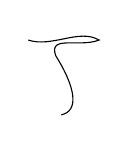
\begin{tikzpicture}[x=1cm,y=1cm]
\draw (0,.55) .. controls (.3,.45) and (.65,.7) .. (.9,.55) .. controls (.65,.45) and (.25,.62) .. (.35,.35) .. controls (.6,-.05) and (.65,-.35) .. (.42,-.4);
\end{tikzpicture}}

\deleted{\unsure{Reprenons} l'\unsure{interprétation} transcendante, et situons donc}
\deleted{\diagram{\begin{tikzcd}
M_g(X) \arrow[dr] & & \operatorname{Conn}(X) \arrow[dl] \\
& M^{\unsure{\xi|\zeta}}_g(X) &
\end{tikzcd}}}

Non, car s'il y en avait, le $\unsure{\xi|\zeta}$-fibré serait associé à un $\unsure{\xi|\zeta}$-fibré affine, donc serait isomorphe à un $P(F)$, où $F$ est une $\unsure{\xi|\zeta}$-extension
\diagram{\begin{tikzcd}
0 \arrow[r,dash] & M \arrow[r] & F \arrow[r] & \mathcal O_X \arrow[r] & 0
\end{tikzcd}}
$M$ est un $\unsure{\xi|\zeta}$-faisceau lin. On aurait donc $E\simeq F\otimes L$, et $\deleted{\unsure{\det}}E\simeq$
% archive foliation: 20
\scanpage{22}
\[
\underset{\substack{\Vert\\\underline{\omega}_X}}{\det E}
\simeq \underset{\substack{\Vert\\M}}{\det F}\otimes L^{\otimes2},
\quad\text{donc }\deleted{\unsure{M\otimes}}\underline{\omega}_X\simeq M\otimes L^{\otimes2}
\]
donc (comme $M$ est de degré $0$) $2\deg L=\deg\underline{\omega}_X$, i.e. \deleted{deg}
\[
\deg L=g-1
\]
Considérons l'hom composé
\deleted{\diagram{\begin{tikzcd}\unsure{\underline{\omega}_X} \arrow[r] & \unsure{E}\end{tikzcd}}}
\diagram{\begin{tikzcd}
\underline{\omega} \arrow[r,hook] & E \arrow[r,"\simeq"{description}] & F\otimes L \arrow[r,two heads] & L
\end{tikzcd}}
d'où une section de $L\otimes\underline{\omega}^{-1}$, qui est de degré $-(g-1)<0$, donc \unsure{elle est} nulle, donc \deleted{cela se factorise par} $E\to L$ se factorise par $E/\underline{\omega}\simeq\mathcal O_X$, donc $L\simeq\mathcal O_X$ absurde car $\deg L\ne0$ !

Ainsi, le \deleted{faisceau} \inserted{groupe} structural du $\unsure{\xi|\zeta}$-fibré projectif associé à une conn. proj. ne peut se réduire à un groupe de Borel.

Montrons qu'il ne peut non plus se réduire à un sous-groupe \unsure{normalisateur} d'un tore maximal. En effet, si cela était le cas, alors par passage à un rev. étale, on se ramènerait au tore maximal, donc à un Borel, absurde (car le genre des revêtements \unsure{ser.} aussi $\geq2$ !). Le même argument montre :

\figure{\begin{tikzpicture}\draw (0,0)--(0,-2.6);\end{tikzpicture}}
\uline{\unsure{Pr.|Prop.}} Soit $X$ courbe projective lisse \inserted{conn.} de genre $g\geq2$ sur corps $k$ (de car nulle ?). Alors pour tte connexion projective sur $X$, on ne \unsure{peut} \deleted{$\unsure{\xi}$} réduire le groupe structural du $\unsure{\xi|\zeta}$-fibré principal de groupe $GP(1)_k=H$ associé, à un sous-groupe \unsure{algéb} $\unsure{H'|H}$ distinct de $H$....
\margin{!}
% archive foliation: 21
\scanpage{23}
Quand $k=\mathbf C$, cela signifie que l'hom correspondant
\diagram{\begin{tikzcd}
\pi_1(X^{\mathrm{an}},x) \arrow[r] & H(\mathbf C)
\end{tikzcd}}
\unsure{à|a} une image Zariski-dense dans $H_{\mathbf C}$.
% archive foliation: 22
\scanpage{25}
\deleted{$h\widehat c=\widehat c$}
\diagram{\begin{tikzcd}[column sep=small]
\left\{\begin{array}{c}(P,\sigma)\\\widehat S\end{array}\right.
\arrow[r,leftrightarrow] & 0 \arrow[r,dash] & \Omega \arrow[r,dash] & E \arrow[r] & \mathcal O_S \arrow[r] & 0
\end{tikzcd}}
$\unsure{\mathcal P|P}$ muni \uline{d'une connexion} $C_P$
\figure{\begin{tikzpicture}[x=1cm,y=1cm]
\draw[->] (0,1.7) .. controls (-.6,1) and (-.4,.7) .. (-.1,.4) .. controls (.1,0) and (.3,0) .. (.7,0) -- (2.9,0) -- (2.9,-.35);
\end{tikzpicture}}
On cherche les iso \inserted{\unsure{étg|etc.}} $\unsure{\mathcal P|P}\xrightarrow{v}\widehat S$ \inserted{(s'il y en a)}, pour lesquels $v(C_P)$ est de la forme $\widehat c$.

La donnée d'un iso. à l'ordre $2$ donne déjà l'extension
\diagram{\begin{tikzcd}[column sep=small]
0 \arrow[r,dash] & \Omega \arrow[r,dash] & E \arrow[r] & \mathcal O_S \arrow[r,dash] & \unsure{0}
\end{tikzcd}}
i.e. définit $(P,\sigma)$ à isom unique près.

Si on se donne \uline{un} isom. entre les $\widehat S$ can. et $\unsure{\mathcal P|P}$, $C_P$ est \unsure{défini} par un $C\in\unsure{\operatorname{Conn}_{\mathrm{proj}}}(\widehat S)$ \inserted{qui prolonge la conn. à l'ordre $2$}. On cherche donc les $g\in G$ (autom \inserted{de $\widehat S$} qui sont l'identité dans l'ordre $2$), tels que $g.C$ de la forme $\widehat c$.

\deleted{\uline{\unsure{Supposons}}} \inserted{Il existe tjrs} \deleted{\unsure{qu'il existe}} un tel $\deleted{\unsure{g_0}}\inserted{\unsure{g'_0|g_0}}$ \deleted{\unsure{à condition}} \inserted{\uline{dès qu'il}} \unsure{y a une connexion} $c_0$ \unsure{sur} $P$, car on aura $gC=h\widehat c_0$
\margin{$(h\in G_0)$ \unsure{unique} \unsure{donc}}
\[
\deleted{g_0C=\widehat c}\quad (h^{-1}g)C=\widehat c_0.
\]
Quels sont les autres ? Ils sont de la forme $g=hg_0$. $(h\in G)$ et la condition est que $gC$ $(=h(g_0C)=h\widehat c)$ soit de la forme $\widehat c'$, i.e. $h\in G_1(c)$.

L'ens de ces $h$ est en correspondance biunivoque avec $\unsure{G/G_0|G_1/G_0}$ -- on peut dire aussi que pour \unsure{tte extension des}
% archive foliation: 24
\scanpage{26}
\uline{\unsure{Th.|Pr.}} Soient $S$ un schéma de car. $0$, $X/S$ un schéma, $\widehat{\mathcal P}=\varprojlim\mathcal P_n$ une \deleted{algèbre} $\mathcal O_X$-Algèbre $\mathcal O_X$-augmentée adique complète, \deleted{\unsure{une}} ($\mathcal J$-adique, \inserted{à filtration adique,} donc $\mathcal J/\mathcal J^2$ \deleted{$\unsure{\simeq\Omega}$} est \uline{inversible}), et muni d'une \deleted{$\unsure{\xi}$} connexion \inserted{\unsure{\deleted{très régulière}|\uline{très régulière}}} $C$ rel. $/S$, respectant la structure d'Algèbre, mais \unsure{non néc.} l'augmentation.
\figure{\begin{tikzpicture}\draw (0,0)--(0,-.8);\end{tikzpicture}}
\inserted{On suppose que l'hom \uuline{lin.} associé
\diagram{\begin{tikzcd}
\mathcal J/\mathcal J^2=\omega \arrow[r,"\bar\omega"] & \Omega^1_{X/S}=\unsure{\widehat S\otimes\Omega^1_{X/S}/\mathcal J\widehat S\otimes\Omega^1_{X/S}}
\end{tikzcd}}
\deleted{\unsure{est}} est un iso. \deleted{(\unsure{conn.} \illegible{3})}}

On cherche les fibrés en droites $P$ sur $X$, munis d'une sect. $\sigma$, (donc défini par extension de \unsure{Mod. loc. lib}
\diagram{\begin{tikzcd}[column sep=small]
0 \arrow[r,dash] & \Omega \arrow[r,dash] & E \arrow[r,dash] & \mathcal O \arrow[r,dash] & 0
\end{tikzcd}}
) muni d'une connexion $c$ (ne respectant pas \unsure{néces.} la section \unsure{marquée|canonique} $\sigma$), \deleted{\unsure{tels}} et les iso d'algèbres augm.
\diagram{\begin{tikzcd}
\widehat S \arrow[r,leftrightarrow,"\substack{u\\\sim}"] & \mathcal P
\end{tikzcd}}
\deleted{tel que} (où $\widehat S=\mathcal O_{\widehat P}$, $\widehat P$ complété formel le long de $\sigma$) tels que $u(\unsure{\widehat C|C})=\widehat c$.

a) La donnée d'un iso $u$ à l'ordre $2$ détermine $(P,\sigma)$, i.e. $\Omega,E$, à isom unique près par
\[
\Omega=\mathcal J/\mathcal J^2,\qquad E=\Omega^{-1}\otimes\mathcal J/\mathcal J^3.
\]
b) $(P,\sigma)$ étant ainsi déterminé, pour tt isom \unsure{alg} à l'ordre $3$ près
\diagram{\begin{tikzcd}
\widehat S/\widehat{\mathcal J}_P^{4} \arrow[r] & \mathcal P/\mathcal J^4
\end{tikzcd}}
prolongeant l'iso à l'ordre $2$ canonique, il existe \uline{un isomorphisme et un seul} $u$ qui le prolonge, et tel que $\unsure{\widehat u|u}(C)$ soit de la forme $\widehat c$, et pour \unsure{tte}
% archive foliation: 25
\scanpage{27}
$c$ \inserted{\unsure{très régulière}} sur $P$ il existe un isom et un seul $u$ \deleted{tel que $u(\widehat c)$} prolongeant $u_3$ et tel que $u(\widehat c)=C$.
\figure{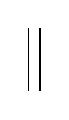
\begin{tikzpicture}\draw (0,0)--(0,-.8);\draw (.15,0)--(.15,-.8);\end{tikzpicture}}
Donc corr. biunivoque entre

a) les solutions du Pb initial, à isom près (NB la cat. des solutions est \uline{rigide})

b) $(P,\sigma)$ étant choisi can. comme expliqué, avec $u_2$, l'ens des \inserted{isom} $u_3$ qui \unsure{prolongent} $u_2$ -- qui forment donc un \inserted{pseudo} torseur sous
\[
\Gamma(X,\Omega^{\otimes2})
\]
c) L'ens des connexions $c$ sur $P$ \deleted{qui} telles que \inserted{$\widehat c$ soit dans} \deleted{soit dans une} une orbite donnée de $G_2$ opérant sur $\operatorname{Conn}^*(P)$, \deleted{\unsure{et qui soit}}

\diagram{\begin{tikzcd}
\operatorname{Iso}^{!}_{\infty} \arrow[d] \arrow[dr] & \\
\operatorname{Sol} \arrow[r,"\sim"] \arrow[dr,"\sim"] & \operatorname{Iso}^{!}_{3} \\
\unsure{\mathrm{rig}} & \operatorname{Conn}^{*}P\;!
\end{tikzcd}}
\[
\deleted{\unsure{u(C)=\widehat c}}\qquad g\widehat c=
\]
\diagram{\begin{tikzcd}
\Omega \arrow[r] & \widehat S\otimes\Omega^1_{X/S}
\end{tikzcd}}
\[
\prod_{i\geq0}\Omega^{\otimes i}\otimes\Omega^1_{X/S}
\]
\[
\Omega^{-1}+\mathcal O+\Omega
\]
\figure{\begin{tikzpicture}[x=.55cm,y=.55cm]
\draw (0,0)--(4.9,3.5)--(6.7,3.8)--(6.9,5)--(10,5.4);
\end{tikzpicture}}
\diagram{\[\begin{array}{cccc}
g\widehat c_0 & \unsure{\widehat c}\quad\deleted{\unsure{\widehat c}}\quad\unsure{\widehat c} & & g\in G(c)\\[1ex]
gu(C_P)=\deleted{\unsure{u(C_P)=\widehat c}} & & gC\unsure{=|:}\widehat c & \\
 u(C)=\widehat c & \unsure{g\widehat c=\widehat c} & \deleted{g\widehat c=C} & g^{-1}\widehat c=C\\[1ex]
 & & u(C_P)=C\unsure{=|:}\widehat c & \\
 & \unsure{gC=g\widehat c} & g\widehat c=\widehat c' & gC=k\widehat c
\end{array}\]}
\diagram{\begin{tikzcd}
\unsure{(gu)(C)=g\widehat c=\widehat c'} \arrow[d,Rightarrow] & & \\
g=\mathrm{id} & h\widehat c=\widehat c \arrow[r,Rightarrow] & |[draw,ellipse]| h=1
\end{tikzcd}}
\[
g\in G(c)
\]
\diagram{\begin{tikzcd}
k^{-1}gC=\widehat c \arrow[dr,dash,bend left=15] & \\
g'C=\widehat c' & \unsure{g'}
\end{tikzcd}}
% archive foliation: 26
\scanpage{28}
\diagram{\begin{tikzcd}
S=\widehat{\operatorname{Sym}}(\Omega) \arrow[r,"C"] & \widehat S\widehat\otimes\Omega^1_{X/S}
\end{tikzcd}}
\diagram{\begin{tikzcd}
\Omega \arrow[r,"C"] & \widehat S\widehat\otimes\Omega^1_{X/S}
\end{tikzcd}}
\[
C(\omega_0)=\sum_{i\geq0}\omega_0^i\otimes\unsure{\varpi_i|\bar\omega_i},\qquad
\unsure{\varpi_i|\bar\omega_i}\in\Omega^1_{X/S}
\]
\[
\begin{aligned}
C(\lambda\omega_0)&=\lambda C(\omega_0)+\omega_0d\lambda\\
&=1\otimes\lambda\unsure{\varpi_0|\bar\omega_0}+\omega_0\otimes(\lambda\unsure{\varpi_1|\bar\omega_1}+d\lambda)+\omega_0^2\otimes\lambda\unsure{\varpi_2|\bar\omega_2}+\cdots\\
&\qquad+\omega_0^i\otimes\lambda\unsure{\varpi_i|\bar\omega_i}\cdots
\end{aligned}
\]
\deleted{$\Omega$}
\diagram{\begin{tikzcd}
\mathcal J^2 \arrow[r,dash] & \mathcal J\otimes\Omega^1_{X/S}
\end{tikzcd}}
\diagram{\begin{tikzcd}
\Omega \arrow[r] & \Omega^1_{X/S}=\Omega
\end{tikzcd}}
\[
d(\lambda\omega)=\lambda d\omega+\underset{\text{nul mod }\mathcal J\otimes\Omega^1_{X/S}}{\deleted{\omega d\lambda}}
\]
\[
\Omega^{-1}\otimes\Omega^1_{X/S}
\]
\diagram{\begin{tikzcd}
\mathcal J^i \arrow[r] & \mathcal J^{i-1}\otimes\Omega^1_{X/S}\\
\lambda\omega^i \arrow[r] & \deleted{C(\omega)}\omega^i\otimes d\lambda+\lambda\omega^{i-1}C(\omega)
\end{tikzcd}}
\deleted{$\unsure{\mathcal P}$}
\diagram{\begin{tikzcd}
\Omega^i \arrow[r,"\mathrm{lin}"] & \Omega^{i-1}\otimes\Omega^1_{X/S}\\
\lambda\omega^i \arrow[r] & \lambda\omega^{i-1}\underline{C(\omega)}\\
\lambda\omega_0^i \arrow[r] & \lambda\omega_0^{i-1}C(\omega_0)
\end{tikzcd}}
\margin{\diagram{\begin{tikzcd}[column sep=small]
C(\omega)= & \unsure{\varpi_0|\bar\omega_0}\omega+\text{termes }\geq1\\
& \Omega^1_{X/S}\otimes\Omega^{-1} \arrow[u]
\end{tikzcd}}}
\figure{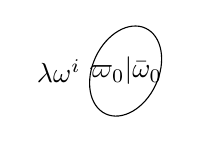
\begin{tikzpicture}
\node at (0,0) {$\lambda\omega^i$};
\node at (.85,0) {$\unsure{\varpi_0|\bar\omega_0}$};
\draw[rotate around={-25:(.85,0)}] (.85,0) ellipse (.42 and .6);
\end{tikzpicture}}
\[
\operatorname{Conn}^{*}
\]
% archive foliation: 27
\scanpage{29}
\[
\begin{aligned}
C(\omega_0^u)^{u^{-1}}={}&\left(\unsure{\varpi_0|\bar\omega_0}+\frac{\omega_0}{1+\sum\alpha_i\omega_0^i}\unsure{\varpi_1|\bar\omega_1}+\left(\frac{\omega_0}{1+\sum\alpha_i\omega_0^i}\right)^2\unsure{\varpi_2|\bar\omega_2}\right)\\
&\cdot\left[1+\sum(i+1)\alpha_i\left(\frac{\omega_0}{1+\sum\alpha_j\omega_0^j}\right)^{\unsure{i}}\right.\unsure{\big]}\\
&+\sum\left(\frac{\omega_0}{\unsure{\sum1+\alpha_j\omega_0^j|1+\sum\alpha_j\omega_0^j}}\right)^{i+1}\otimes d\alpha_i.
\end{aligned}
\]
Supposons $\alpha_2=0$, et calculons mod $\Omega^4$
\[
\begin{aligned}
C(\omega_0^u)^{u^{-1}}
&\underset{\substack{\mathrm{mod}\\\sum_{i\geq4}\Omega^i\otimes\Omega^1_{X/S}}}{\equiv}
(\unsure{\varpi_0|\bar\omega_0}+\omega_0\unsure{\varpi_1|\bar\omega_1}+\omega_0^2\unsure{\varpi_2|\bar\omega_2})
[1+\deleted{\unsure{(i+1)\alpha_i}}\inserted{4\alpha_3\omega_0^3}]\\
&\unsure{+}\\
&=\deleted{\unsure{\varpi_2}}C(\omega_0)+4\alpha_3\omega_0^3\unsure{\varpi_0|\bar\omega_0}
\end{aligned}
\]
\margin{il faut $\alpha_3=0$}
Supposons $\alpha_2=0\quad\unsure{\alpha_{n-1}|\alpha_n}=0$ $(n\geq3)$ calculons mod $\Omega^{n+1}$
\inserted{$\alpha_n=?$}
\[
\begin{aligned}
C(\omega_0^u)^{u^{-1}}&=(\unsure{\varpi_0|\bar\omega_0}+\omega_0\unsure{\varpi_1|\bar\omega_1}+\omega_0^2\unsure{\varpi_2|\bar\omega_2})(1+(n+1)\alpha_n\omega_0^n)\\
&=\deleted{\unsure{\varpi_0}}C(\deleted{\unsure{\omega}}\omega_0)+\deleted{\unsure{\varpi_0\lambda}}\underline{(n+1)\alpha_n\omega_0^n}\unsure{\varpi_0|\bar\omega_0}
\end{aligned}
\]
donc il faut $(n+1)\alpha_n=0$.

Calculons mod $\Omega^3$ en \inserted{ne} \unsure{supposant plus} $\alpha_2$,
Je trouve
\[
\begin{aligned}
C(\omega_0^u)^{u^{-1}}&=(\unsure{\varpi_0|\bar\omega_0}+\omega_0\unsure{\varpi_1|\bar\omega_1}+\omega_0^2\unsure{\varpi_2|\bar\omega_2})(1+3\alpha_2\omega_0^2)\\
&=C(\omega_0)+\underline{3\alpha_2}\omega_0^2\underline{\unsure{\varpi_0|\bar\omega_0}}
\end{aligned}
\]
\uline{Prop.} Soit \inserted{$\operatorname{Conn}(P)$} l'ens des connexions \inserted{$c$} de $P$ (ou de l'Alg. \inserted{de Lie} $(\unsure{H|\mathfrak g})$), \deleted{\unsure{soit}} $G_0$ \deleted{l'ens} groupe des autom $u$ de $\widehat S$ \inserted{(alg. augm.)} (qui sont l'identité mod $\unsure{\mathcal J^4|\mathcal J^3}$), considérons l'application
\diagram{\begin{tikzcd}
(c,u) \arrow[r,maps to] & \deleted{\unsure{\widehat c}}\deleted{\unsure{u\widehat c}}u(\widehat c)\\
\operatorname{Conn}P\inserted{\times G_0} \arrow[r] & \operatorname{Conn}_{\unsure{\Omega_0|\omega_0}}(\widehat S)\deleted{\unsure{\mathrm{mod}}}
\end{tikzcd}}
\figure{\begin{tikzpicture}\draw (0,0)--(0,-2.7);\end{tikzpicture}}
\uline{Cette application est bijective} ($\unsure{X|S}$ de car. $0$)
% archive foliation: 28
\scanpage{30}
\uline{Cor} Supposons $u\in G_0$, \deleted{$\unsure{u\widehat c}$} et $u\widehat c$ de la forme $\widehat c'$
\uline{Alors} $u=\mathrm{id}$

En effet, $\deleted{\unsure{u\widehat c}}$ \uuline{$u.\widehat c=1.\widehat c'$} $\Rightarrow\ (u,c)=(1,c')$

Soit $G$ le groupe des autom \unsure{\deleted{qui}|qui} de $\widehat S$ qui sont l'identité mod $\mathcal J^3$ (donc $G/G_0\sim\Gamma(\Omega^{\otimes2})$) et considérons $(g,c)\longmapsto g.\widehat c$ sur $G\times\operatorname{Conn}(P)$. Quand a-t-on
\[
g\widehat c=g'\widehat c',\quad\text{i.e. }(g'^{-1}g)\widehat c=c'\quad\text{i.e. }h\widehat c=\widehat c'
\]
quand $h\widehat c$ est-il de la forme $\widehat c'$ ?

\inserted{Alors $c$ fixé, on trouve} \deleted{C'est} un sous-ensemble $G(c)$ de $G$
\[
h\in G(c)\quad\Longleftrightarrow\quad h.\widehat c\text{ de la forme }\widehat c'
\]
\deleted{$h\in G(c),\ g\in G_0,\ gh\in G(c)$}
On trouve que
\deleted{$\Rightarrow g=1$, donc pour $G(c)$}
\deleted{$G(c)\times$}
\diagram{\begin{tikzcd}
G_0\times G(c) \arrow[r] & G\\
(g,h) \arrow[r,maps to] & g.h
\end{tikzcd}}
est bijectif,

(si $gh=g'h'$ i.e. $\underbrace{(g'^{-1}g)}_{g''}h=h'$

d'où $\deleted{(g'^{-1}g)}\ (g''h).\widehat c$ de la forme $\widehat c''$
\[
\begin{array}{c}
\Vert\\
g''(\underbrace{h\widehat c}_{\widehat c'})
\end{array}
\]
D'où $g''=1$, d'où $\deleted{\unsure{g''}}\ g=g'$ et par suite $h=h'$.

\deleted{Inversement,} Surjectif, car soit $g\in G$
\diagram{\begin{tikzcd}[column sep=small]
\text{on a }g\widehat c= & k\widehat c' & \text{d'où } k^{-1}g\unsure{=|\equiv}h\in G(c)\\
& G_0 \arrow[u] &
\end{tikzcd}}
d'où $g=kh$
% archive foliation: 29
\scanpage{31}
\[
\begin{aligned}
C(\omega^u)&=\deleted{\unsure{\omega+\omega}}\ C\omega+\sum_{i\geq2}C(\omega)u_i+\omega C(u_i)\\
&=C(\omega)(1+\sum_{i\geq2}u_i)+\omega\sum C(u_i).
\end{aligned}
\]
\deleted{Prenons}
\[
C\upharpoonright\Omega:\quad\Omega\xrightarrow{C}\widehat S\otimes\Omega^1_{X/S}
\qquad C(\omega)=\unsure{\omega_{-1}+\omega\omega_0+\omega\omega_1|\varpi_{-1}+\omega\varpi_0+\omega\varpi_1}.
\]
\[\Omega^{\otimes i}\]
\[
C(\lambda\omega^{\otimes i})=
\deleted{\omega^{\otimes i}\otimes d\lambda+\lambda i\omega^{\otimes(i-1)}}
\quad\underbrace{\omega^i\otimes d\lambda+\lambda i\omega^{i-1}(\unsure{\omega_{-1}+\omega_0\omega_1|\varpi_{-1}+\omega\varpi_1})}.
\]
\[\omega=\lambda\omega_0\qquad u_i=\deleted{\unsure{\alpha_i\omega_0^i}}\alpha_i\omega_0^i.\]
\[
\begin{aligned}
C((\lambda\omega_0)^u)&=(\lambda\deleted{C(\omega)}\inserted{C(\omega_0)}+\omega_0\otimes d\lambda)(1+\sum_{i\geq2}\alpha_i\omega_0^i)\\
&\quad+\lambda\omega_0\sum_{i\geq2}(\omega_0^i\otimes d\alpha_i+i\alpha_i\omega_0^{i-1}C(\omega_0)).
\end{aligned}
\]
\[
C(\omega_0)=\deleted{\unsure{\varpi_0+\varpi_1+\varpi_2}}
\inserted{\unsure{\varpi_0|\bar\omega_0}+\omega_0\unsure{\varpi_1|\bar\omega_1}+\omega_0^2\unsure{\varpi_2|\bar\omega_2}}
\qquad\unsure{\varpi_i|\bar\omega_i}\in\deleted{\unsure{\Omega}}\ \Omega^1_{X/S}.
\]
\[
C(\deleted{\lambda}\omega_0^u)=\deleted{C(\omega_0)}(\unsure{\varpi_0+\varpi_1+\varpi_2})(1+\sum_{i\geq2}\alpha_i\omega_0^i+\sum_{i\geq2}i\alpha_i\omega_0^{\unsure{i|i-1}}).
\]
\[
\begin{aligned}
C(\omega_0^u)&=C(\omega_0(1+\sum_{i\geq2}\alpha_i\omega_0^i))\\
&=C(\omega_0)(1+\sum\alpha_i\omega_0^i)\\
&\quad+\omega_0\sum_{i\geq2}(\omega_0^i\otimes d\alpha_i+i\alpha_i\omega_0^{i-1}C(\omega_0))\\
&=C(\omega_0)(1+\sum_{i\geq2}(i+1)\alpha_i\omega_0^i)+\omega_0^3\sum_{i\geq2}\omega_0^{i-2}\otimes d\alpha_i\\
&=(\unsure{\varpi_0+\varpi_1+\varpi_2})(\qquad\text{''}\qquad)+\qquad\text{''}
\end{aligned}
\]
\[\deleted{\unsure{C(\omega_0^u)^{u^{-1}}=C(1+\sum_{i\geq2}}}\]
\[
\begin{aligned}
C(\omega_0^u)^{u^{-1}}&=\unsure{C(\omega_0)^{u^{-1}}}
\left(1+\sum_{i\geq2}(i+1)\alpha_i\left(\frac{\omega_0}{1+\sum\alpha_j\omega_0^j}\right)^i\right)\\
&\quad+\deleted{\omega_0}\sum_{i\geq2}\left(\frac{\omega_0}{1+\sum_{j\geq2}\alpha_j\omega_0^j}\right)^{i+1}\otimes d\alpha_i.
\end{aligned}
\]
\[
\deleted{C(\omega_0)^{u^{-1}}=\unsure{\varpi_0|\bar\omega_0}+\frac{\unsure{\varpi_1|\bar\omega_1}}{\unsure{1+\sum\alpha_j\omega_0^j}}+\omega_0^{u^{-1}}\unsure{\varpi_2|\bar\omega_2}}.
\]
\figure{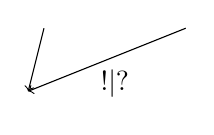
\begin{tikzpicture}[x=1cm,y=1cm]\node at (0.9,0) {$\unsure{!|?}$};\draw[->] (0,0.7)--(-0.2,-0.1);\draw[->] (1.8,0.7)--(-0.2,-0.1);\end{tikzpicture}}
% archive foliation: 30
\scanpage{32}
\[G\supset G_0\qquad C\supset C_0\]
$G$ gpe, $G_0$ ss-gpe, \deleted{\unsure{invariant}}

$C$ $G$-ens, $C_0$ sous-ens
\diagram{\begin{tikzcd}
G_0\times C_0\arrow[r,"\sim"] & C\\
(h,c)\arrow[r,mapsto] & h.c
\end{tikzcd}}
Soit $c\in C_0$, et soit
\[G(c)=\{g\in G\mid g.c\in C_0\}.\]
Alors $G(c)\xrightarrow{\sim}{}_{G_0}\backslash G\deleted{/G_0}$ i.e.

\deleted{En effet,}
\deleted{
\diagram{\begin{tikzcd}
G_0\times G(c)\arrow[r,"\sim"] & G\\
(h,g)\arrow[r,mapsto] & h.g
\end{tikzcd}}
En effet, si $hg=h'g'$, \quad $h,h'\in G_0$, $g,g'\in G(c)$,
\[
\underbrace{(h'^{-1}h)}_{h''}g=g'\quad\text{d'où}\quad
h''\underbrace{(gc)}_{\substack{\uparrow\\C_0}}=\underbrace{g'c}_{\substack{\uparrow\\C_0}}=1.\underbrace{(g'c)}_{\substack{\uparrow\\C_0}}
\]
donc $h''=1$ i.e. $h=h'$ et $g=g'$, d'où l'injectivité.
}
\margin{\unsure{Si}\ $\leftrightarrow$}
\margin{\uline{Cor} ${}_{G_0}\backslash C\simeq C_0$ (bij. ens abstraits).
\uline{Rem.} (\unsure{Si $G_0$ inv. dans $G$}) $G/G_0$ opère sur $C_0$, $C/G\simeq C_0/(G/G_0)$.}
Surjectivité: Soit $k\in G$, alors $kc\in C$ de la forme $h'c'$
($h'\in G_0$, $c'\in C_0$) donc $\underbrace{h'^{-1}k}_{g}c=c'$,
donc $h'^{-1}k=g\in G(c)$ donc
\[k=h'g,\quad h'\in G_0,\quad\uline{g\in G(c)}.\]
\unsure{Q.S.}\ \deleted{\unsure{Soit}} $g\in G$, $c\in C_0$, $gc=c\Longrightarrow g=1$ ?

\deleted{On aura $g\in G(c)$, $1\in\unsure{G}$}

Considérons une orbite de $G$ dans $C$, soit $G.x$, et considérons $O\cap C_0$. Alors
\[O\cap C_0\simeq\deleted{\unsure{C/}}{}_{G_0}\backslash G.\]
En effet, \unsure{si}
\[x=h.\hat c_0\quad(h\in G_0,\ c_0\in C_0,\text{uniques})\quad\text{donc}\]
\[\deleted{\unsure{nous}\ \unsure{\mathrm{WTS}}\ g\inserted{x}\in G_0\unsure{\longmapsto h}\quad g.h.c}\]
% archive foliation: 31
\scanpage{33}
$X/S$ schéma relatif

$\mathcal P$: $\mathcal O_X$-Algèbre augmentée, sép. complète pour la top. $J$-adique ($J$ idéal d'augmentation)
\inserted{$J/J^2=\Omega$ inv.}
\[
C:\mathcal P\longrightarrow\mathcal P\widehat\otimes\Omega^1_{X/S}
\]
connexion \inserted{d'Algèbre} (ne \unsure{respectant} pas néc. l'augmentation)
\[
\begin{cases}
C(fg)=fC(g)+gC(f)& f,g\text{ sections de }\mathcal P\\
C(\lambda.1)=1\otimes d\lambda&\lambda\text{ section de }\mathcal O_X.
\end{cases}
\]
\deleted{\unsure{Comment peut-on connaître $C$}}

\uline{N.B.} Localt (sur des ouverts affines) \deleted{On a}
\deleted{\unsure{pour}} iso $\mathcal P\simeq\widehat{\operatorname{Sym}}(\Omega)$ (\unsure{compatibles aux augm.}) et $C$ connu quand on connaît
$C|\Omega$, qui est un hom. \uline{additif}
\[
\Omega\longrightarrow\widehat{\operatorname{Sym}}(\Omega)\widehat\otimes\Omega^1_{X/S}
=\prod_{i\geq0}\underbrace{\operatorname{Sym}^i(\Omega)}_{\Omega^{\otimes i}}\otimes\Omega^1_{X/S}
\qquad C_\Omega=(\unsure{\varpi_i|\bar\omega_i})
\]
où les $\unsure{\varpi_i|\bar\omega_i}$ pour $i\neq1$ sont \uline{linéaires}, et
$\unsure{\varpi_1|\bar\omega_1}$ est une connexion de modules --- les $\unsure{\varpi_i|\bar\omega_i}$ par ailleurs quelc. On interprète
\[
\begin{cases}
\unsure{\varpi_i|\bar\omega_i}\in\deleted{\unsure{\Gamma\operatorname{Sym}^i}}\Gamma\,\Omega^{\otimes(i-1)}\otimes\Omega^1_{X/S}&(i\neq1)\\
\unsure{\varpi_1|\bar\omega_1}\text{ une connexion sur }\Omega.
\end{cases}
\]
On voit sur ceci que $C$ \unsure{satisfait tjrs à}
\[C(J^i)\subset J^{i-1}\widehat\otimes\Omega^1_{X/S}\]
donc $C$ induit un hom. $(i\geq1)$
\[
\operatorname{gr}^i(\mathcal P)=J^i/J^{i+1}\simeq\Omega^i
\xrightarrow{\deleted{\unsure{C}}\inserted{\widetilde C}}
\unsure{\operatorname{gr}^{i-1}}(\mathcal P\widehat\otimes\Omega^1_{X/S})
\quad\begin{matrix}\simeq\\\Omega^{i-1}\otimes\Omega^1_{X/S}\end{matrix}
\]
qui est tjrs \inserted{$\mathcal O_S$-}\uline{linéaire}, et $\unsure{=|\text{est}}$
$\operatorname{Sym}(\Omega)$-linéaire, donné par
\[\widetilde C(\omega_{\unsure{i|0}})=\omega_i\otimes\unsure{\varpi_0|\bar\omega_0}.\]
% archive foliation: 32
\scanpage{34}
où
\[\unsure{\varpi_0|\bar\omega_0}\in\Gamma(\Omega^{-1}\otimes\Omega^1_{X/S})=\operatorname{Hom}(\Omega,\Omega^1_{X/S})\]
est indépendant de $i$, et est le $\unsure{\varpi_0|\bar\omega_0}$ de tout à l'heure pour un splitting. On dit que $C$ est connexion \uline{régulière} si la section $\unsure{\varpi_0|\bar\omega_0}$ de $\Omega^{-1}\otimes\Omega^1_{X/S}$ est \uline{régulière}.

\deleted{(\unsure{terme que nous utiliserons par la suite sans autres})}
\inserted{très régulière si} \deleted{\unsure{l'on a}}
\[\unsure{\varpi_0|\bar\omega_0}:\Omega\xrightarrow{\sim}\Omega^1_{X/S}\quad!\quad)\]
\uline{Prop} \inserted{(car. nulle)} Supposons
\[\mathcal P=\widehat S=\mathcal O_{\widehat P},\quad\text{où }(P,\sigma)\]
associé à une suite ex. de $0\longrightarrow\Omega\longrightarrow E\longrightarrow\mathcal O_X\longrightarrow0$.

Soit \deleted{\unsure{Supposons}} $\operatorname{Conn}(P)\deleted{\unsure{^{*}}}$ l'ens des conn. \deleted{\unsure{régulières}} $c$ de $P$, \deleted{telles que $\hat c$} $\operatorname{Conn}(\widehat S)$ \inserted{l'ens des} conn. de $\widehat S$, d'où $c\longmapsto\hat c$
\[\operatorname{Conn}(P)\longrightarrow\operatorname{Conn}(\widehat S)\]
et soit $\operatorname{Conn}^{*}(\widehat S)\subset\operatorname{Conn}(\widehat S)$ formé des conn. \uline{régulières} \inserted{(\unsure{ou très régt|un peu fort})} de $\widehat S$, $\operatorname{Conn}^{*}(P)$ son image inverse dans $\operatorname{Conn}(P)$. Soit $G$ ($G_0$) le gpe des auto de $\widehat S$ augmenté qui sont l'identité mod $J^3$ ($J^4$).

\inserted{Alors,} L'application
\diagram{\begin{tikzcd}
\operatorname{Conn}^{*}(P)\times G_0\arrow[r] & \operatorname{Conn}^{*}(\widehat S)\\
(c,g)\arrow[r,mapsto] & g.\hat c
\end{tikzcd}}
est \unsure{bijective|injective} (\unsure{resp.|unq.} bijective)
\margin{De plus, \unsure{l'action de $G_0$ dans $\operatorname{Conn}^{*}(\widehat S)$} \deleted{\unsure{de}\ \illegible{2}} \unsure{est libre}.}
\figure{\begin{tikzpicture}[x=1cm,y=1cm]
\draw (0.8,2.6) .. controls (.65,1.9) and (.65,1.1) .. (.9,.95) .. controls (1.5,.6) and (1.6,1.3) .. (.9,.95) .. controls (.65,.75) and (.65,.35) .. (.65,0);
\draw[->] (-1.2,-.25)--(-.8,-.25);
\end{tikzpicture}}
\uline{Cor} \inserted{Soit $c\in\operatorname{Conn}^{*}(P)$,}
L'ens $G(c)\subset G$ des $g\in G$ tels que
\[g\hat c\in\operatorname{Im}\operatorname{Conn}^{*}(P)\]
est tel que
\[
G(c)\xrightarrow{\sim}G/G_0\quad\begin{matrix}\simeq\\\Gamma(X,\Omega^{\otimes2})\end{matrix}
\]
% archive foliation: 33
